\documentclass[UTF8]{ctexart}
\usepackage{graphicx} % Required for inserting images
\usepackage{amsmath}
\usepackage{listings}
\usepackage{color}

\definecolor{dkgreen}{rgb}{0,0.6,0}
\definecolor{gray}{rgb}{0.5,0.5,0.5}
\definecolor{mauve}{rgb}{0.58,0,0.82}

\lstset{frame=tb,
	language=Python,
	aboveskip=3mm,
	belowskip=3mm,
	showstringspaces=false,
	columns=flexible,
	basicstyle={\small\ttfamily},
	numbers=none,
	numberstyle=\tiny\color{gray},
	keywordstyle=\color{blue},
	commentstyle=\color{dkgreen},
	stringstyle=\color{mauve},
	breaklines=true,
	breakatwhitespace=true,
	tabsize=3
}

\pagestyle{plain}	%取消页眉
\usepackage{fontspec}
\usepackage{geometry}
\usepackage{float}   %H选项打开
\addtocounter{MaxMatrixCols}{10} %矩阵列数大于10
\title{RL Homework 2}
\author{20241202239}
\date{September 2024}
\begin{document}
	
	\maketitle
	\paragraph{Language:} Python
	
	\paragraph{Problem setup:}
	\textbf{Environment:} 4*4 grid world.
	\textbf{Reword:} is $r_{boundary} = r_{forbidden}=-1$, and $r_{target}=1$. 
	\textbf{Discount rate:} is $\gamma =0.9$

	\paragraph{Understanding of this algorithm:} There are two steps in value  iteration: first is \textit{policy update}, it aims to fin new policy that $\pi_{k+1} = arg \textbf{ }max(r_{\pi} + \gamma P_{\pi}v_k)$, second is \textit{value update}, calculate new state value from updated policy, $v_{k+1} = r_{\pi_{k+1}} + \gamma P_{\pi_{k+1}}v_k$.
	\paragraph{Key parts of code:}
	\begin{lstlisting}		
		def update_P(policy): #update martrix by policy
		    P = np.zeros((16,16))
		    for i in range(16):
		        if i in [6,9,14]: #pass forbidden
		            continue
		        if policy[i] == 1:
		            if ((i//4)==3)|((i+1) in [6,9,14]):
		                P[i][i] = 1
		            else:
		                P[i][i+1] = 1
		        elif policy[i] == 0:
		            if (i>11)|((i+4) in [6,9,14]):
		                P[i][i] = 1
		            else:
		                P[i][i+4] = 1
		        elif policy[i] == 3:
		            if ((i//4)==0)|((i-1) in [6,9,14]):
		                P[i][i] = 1
		            else:
		                P[i][i-1] = 1
		        elif policy[i] == 2:
		            if (i<4)|((i-4) in [6,9,14]):
		                P[i][i] = 1
		            else:
		                P[i][i-4] = 1
		        elif policy[i] == 4:
		            P[i][i] = 1
		
		    P = np.delete(P, [6,9,14], axis=0)  
		    P = np.delete(P, [6,9,14], axis=1)
		
		    return P
		
		if __name__ == "__main__":      
		    discount=0.9
		
		    policy = np.ones(16,dtype=int)
		    P = update_P(policy)
		  
		    state_value = np.zeros((16,1)) #initial values
		    for i in range(61): #iteration
		        env = GridWorld(env_size = (4,4),start_state = (0,0),target_state = (2,2),
		                    forbidden_states = [(2,1),(1,2),(2,3)],reward_target=1,
		                    reward_forbidden=-1,reward_step=0)
		        state = env.reset()
		        rpi = []
		        for s in range(16):  
		            if s in [6,9,14]:
		                continue
		            q_table = []
		            for k in range(5): #k is action
		                (x, y), reward = env._get_next_state_and_reward((s%4,s//4),env.action_space[k])
		                q_table.append(reward+discount*(state_value[y*4+x]))  
		            max_value = max(q_table) #get q_table and choose firdt max valueas update action
		            
		            policy[s] = q_table.index(max_value)
		            (x, y), reward = env._get_next_state_and_reward((s%4,s//4),env.action_space[policy[s]])
		
		            rpi.append(reward) #update return
		        #state_value update
		        P = update_P(policy)
		        state_value = np.delete(state_value, [6,9,14])
		        state_value = 0.9*P@state_value + rpi
		        state_value = np.insert(state_value,6,0)
		        state_value = np.insert(state_value,9,0)
		        state_value = np.insert(state_value,14,0)
	\end{lstlisting}
	Initially, set the all state value is zero, than calculate q-values for every state, choose the action with greatest q-values to update policy, than we use new policy to update state value for iteration.
	\paragraph{Optimal policy and optimal state values:}
	Here plot the policy:
	\begin{figure}[H]
			\centering
				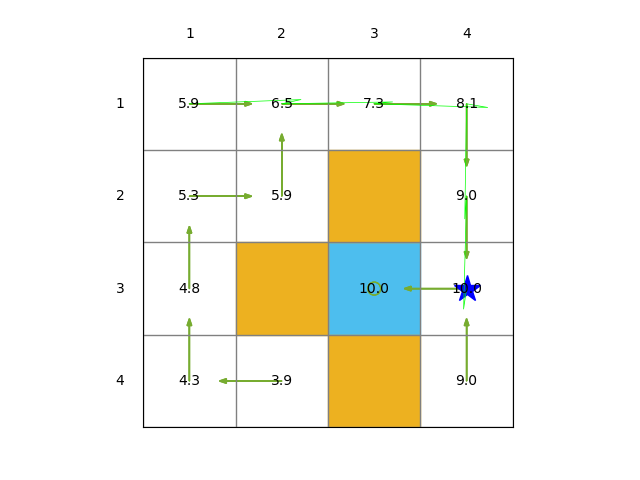
\includegraphics[width=6cm,height=6cm]{fig/policy1}
				\caption{Optimal Policy}
	\end{figure}
	
	\subparagraph{Evolvement:} There are 61 iteration,  first five and the last five figures are plot.
	\begin{figure}[H]
			\centering
			\begin{minipage}[t]{0.3\textwidth}
				\centering
				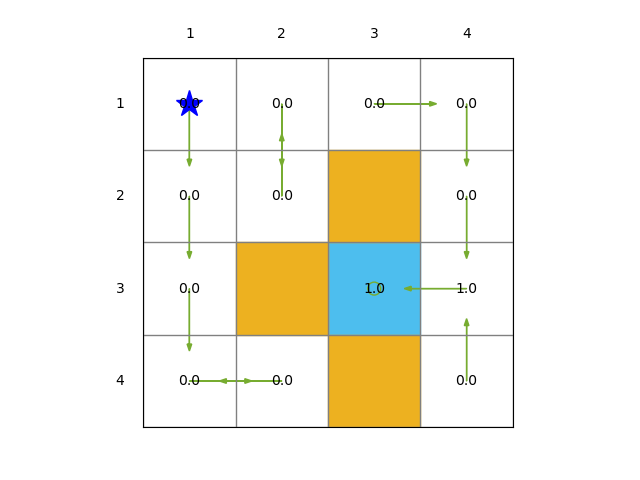
\includegraphics[width=4cm,height=3cm]{fig/PolicyAndState_0}
				\caption{k=1}
			\end{minipage}
			\begin{minipage}[t]{0.3\textwidth}
				\centering
				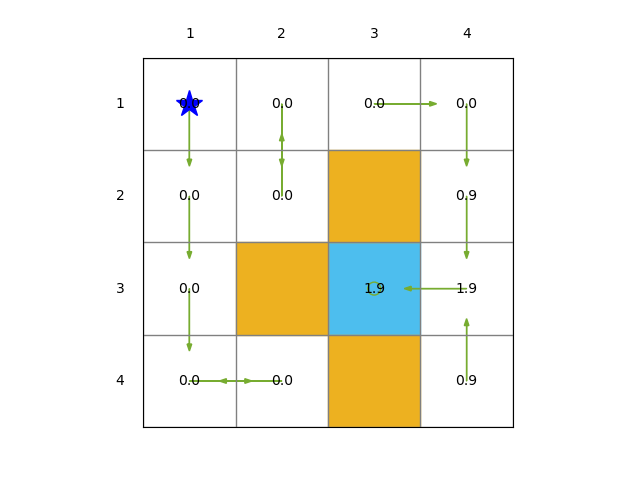
\includegraphics[width=4cm,height=3cm]{fig/PolicyAndState_1}
				\caption{k=2}
			\end{minipage}
			\begin{minipage}[t]{0.3\textwidth}
				\centering
				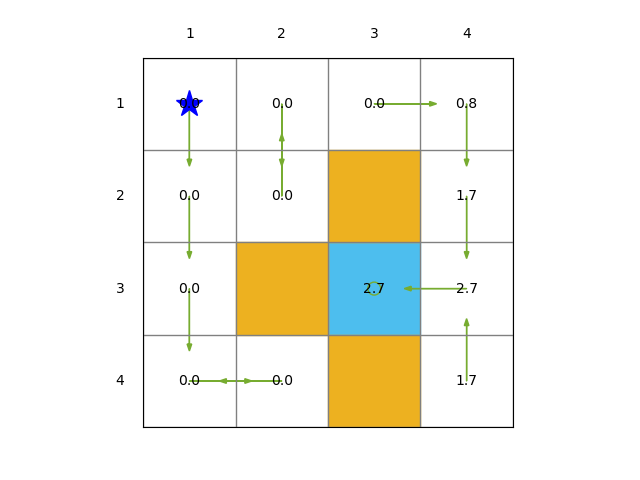
\includegraphics[width=4cm,height=3cm]{fig/PolicyAndState_2}
				\caption{k=3}
			\end{minipage}
		\end{figure}
	\begin{figure}[H]
		\centering
		\begin{minipage}[t]{0.45\textwidth}
			\centering
			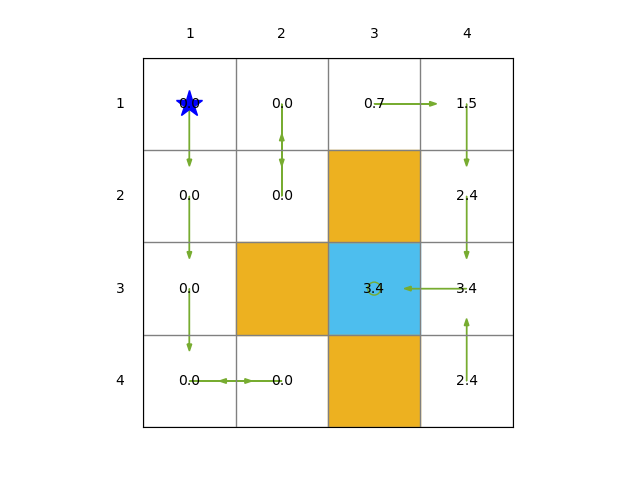
\includegraphics[width=4cm,height=3cm]{fig/PolicyAndState_3}
			\caption{k=4}
		\end{minipage}
		\begin{minipage}[t]{0.45\textwidth}
			\centering
			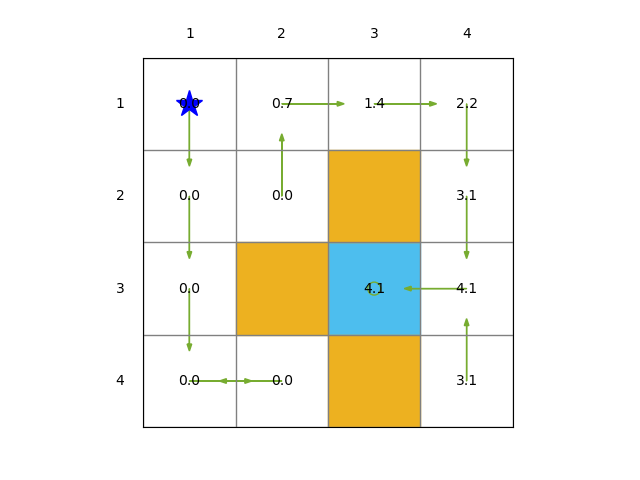
\includegraphics[width=4cm,height=3cm]{fig/PolicyAndState_4}
			\caption{k=5}
		\end{minipage}
	\end{figure}
	\begin{figure}[H]
		\centering
		\begin{minipage}[t]{0.3\textwidth}
			\centering
			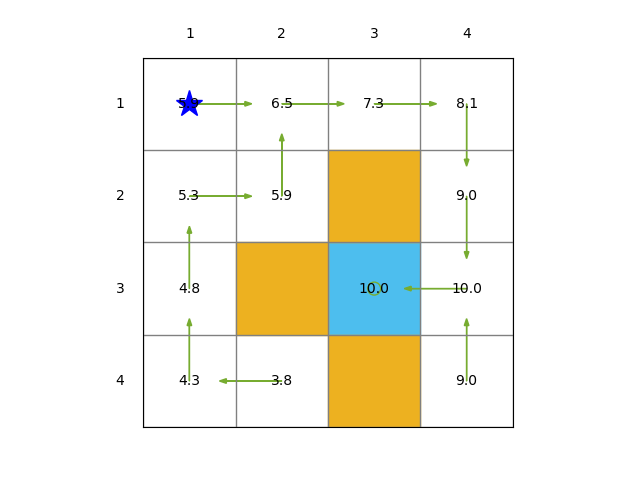
\includegraphics[width=4cm,height=3cm]{fig/PolicyAndState_56}
			\caption{k=57}
		\end{minipage}
		\begin{minipage}[t]{0.3\textwidth}
			\centering
			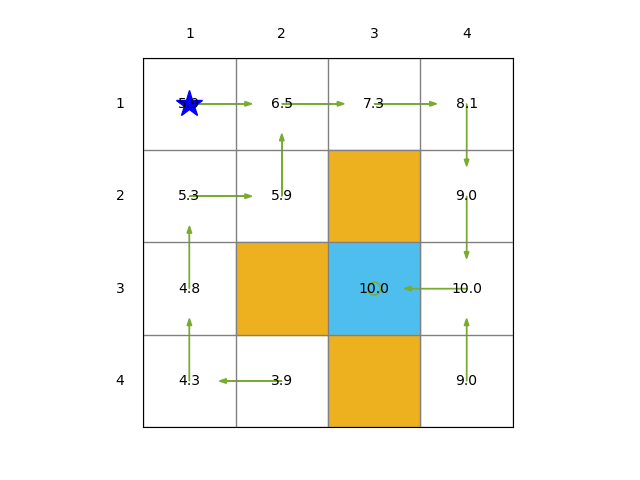
\includegraphics[width=4cm,height=3cm]{fig/PolicyAndState_57}
			\caption{k=58}
		\end{minipage}
		\begin{minipage}[t]{0.3\textwidth}
			\centering
			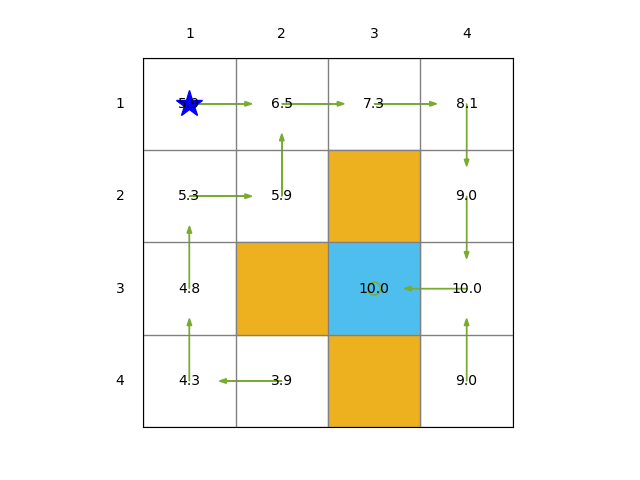
\includegraphics[width=4cm,height=3cm]{fig/PolicyAndState_58}
			\caption{k=59}
		\end{minipage}
	\end{figure}
	\begin{figure}[H]
		\centering
		\begin{minipage}[t]{0.45\textwidth}
			\centering
			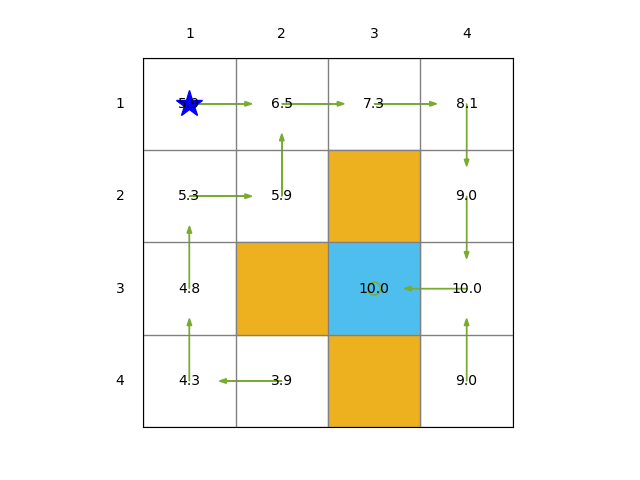
\includegraphics[width=4cm,height=3cm]{fig/PolicyAndState_59}
			\caption{k=60}
		\end{minipage}
		\begin{minipage}[t]{0.45\textwidth}
			\centering
			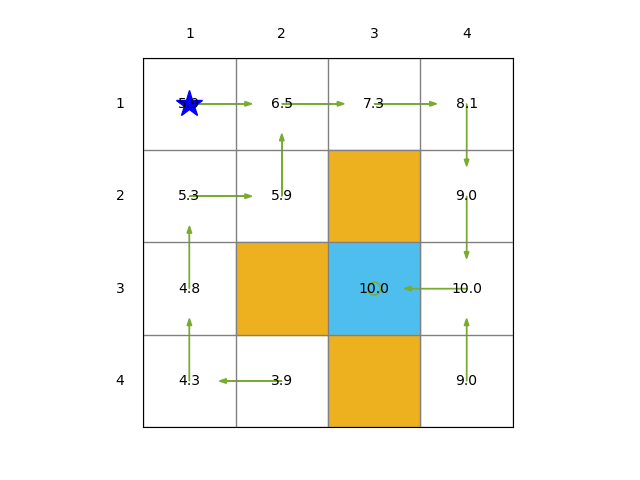
\includegraphics[width=4cm,height=3cm]{fig/PolicyAndState_60}
			\caption{k=61}
		\end{minipage}
	\end{figure}
	\paragraph{Observation} The iteration firstly update the state value form the target, and then nearby state. After policy is fixed, state value are still update like use iterative solution to find state value for a policy.

\end{document}